% CVPR 2022 Paper Template
% based on the CVPR template provided by Ming-Ming Cheng (https://github.com/MCG-NKU/CVPR_Template)
% modified and extended by Stefan Roth (stefan.roth@NOSPAMtu-darmstadt.de)

\documentclass[10pt,twocolumn,letterpaper]{article}

%%%%%%%%% PAPER TYPE  - PLEASE UPDATE FOR FINAL VERSION
\usepackage[review]{cvpr}      % To produce the REVIEW version
%\usepackage{cvpr}              % To produce the CAMERA-READY version
%\usepackage[pagenumbers]{cvpr} % To force page numbers, e.g. for an arXiv version

% Include other packages here, before hyperref.
\usepackage{graphicx}
\usepackage{amsmath}
\usepackage{amssymb}
\usepackage{booktabs}
\usepackage{multirow}


% It is strongly recommended to use hyperref, especially for the review version.
% hyperref with option pagebackref eases the reviewers' job.
% Please disable hyperref *only* if you encounter grave issues, e.g. with the
% file validation for the camera-ready version.
%
% If you comment hyperref and then uncomment it, you should delete
% ReviewTempalte.aux before re-running LaTeX.
% (Or just hit 'q' on the first LaTeX run, let it finish, and you
%  should be clear).
\usepackage[pagebackref,breaklinks,colorlinks]{hyperref}


% Support for easy cross-referencing
\usepackage[capitalize]{cleveref}
\crefname{section}{Sec.}{Secs.}
\Crefname{section}{Section}{Sections}
\Crefname{table}{Table}{Tables}
\crefname{table}{Tab.}{Tabs.}


%%%%%%%%% PAPER ID  - PLEASE UPDATE
\def\cvprPaperID{Group 7} % *** Enter the CVPR Paper ID here
\def\confName{ECE 251C}
\def\confYear{Fall 2021}


\begin{document}

%%%%%%%%% TITLE - PLEASE UPDATE
\title{Feature Extraction of ECG signals using Wavelet transform}

\maketitle

%%%%%%%%% ABSTRACT
\begin{abstract}
Electrocardiograms (ECG) are signals which capture the mechanical activity of the heart. These signals are usually fairly periodic and they provide first-hand insights into any cardiovascular abnormalities or diseases that a person might have in the future. We can take advantage of the periodicity of these signals to classify various heart-related conditions depending upon the variations which these ECG signals undergo. This project discusses two such methods to perform binary classification of ECG signals between healthy and unhealthy ones. Specifically, we take the concepts of wavelets and wavelet packet decomposition to extract features from these signals by performing mathematical operations on them and feeding that extracted feature data to the Machine Learning based classifier. Finally, we would want to come to a conclusion about the most suitable classifier, decomposition level, and wavelet combination.\\
   \providecommand{\keywords}[1]
{
  \small	
  \textbf{\textit{Keywords---}} #1
}
\keywords{DWT - Discrete Wavelet Transform, WPD - Wavelet Packet Decomposition, ECG - Electrocardiogram, SVM - Support Vector Machine, KNN - k-Nearest Neighbours, Db - Daubechies}
\end{abstract}

%%%%%%%%% BODY TEXT
\section{Introduction}
\label{sec:intro}
In today’s age Rising Cardiovascular diseases, pegs need of timely diagnosis. Apart from regular health checkups, an easy \& accessible heart health diagnosis solution is needed to prevent mishaps like heart failure. One such solution can be - to use the pulse data (similar to ECG data) from wearable health monitoring devices like Fitbit and analyze that data to detect/diagnose an early warning sign which will enable us to predict the onset of cardiovascular disease. There are various factors which we would have to incorporate such a system – like the power consumption, performance, precision of measurement, desired accuracy of the predictions, etc.
Now, to build a full ECG abnormality detection and classification mechanism, we would have to choose and implement proper techniques to perform the following actions- data preprocessing, feature extraction, and classification. In this project, our main focus would be on the feature extraction step of this design and the usage of wavelet decomposition and analysis techniques - namely - Discrete Wavelet Transform (DWT) and Wavelet Packet Decomposition (WPD) for the feature extraction of ECG signals.
To see how effective DWT and WPD feature extraction techniques are with respect to different classifiers and what impact do they have on classification accuracy, we have performed the experiment where we vary the scale(5,9,10), mother wavelet type (db4, db6, haar, symlet4), technique( DWT/ WPD) and classifier(SVM, KNN, Fine decision Tree)  to obtain the best working combination of these to maximize the accuracy of the system.
Figure 1 shows the difference between a Healthy ECG signal and an unhealthy ECG signal that has arrhythmia.
\begin{figure}[h!]
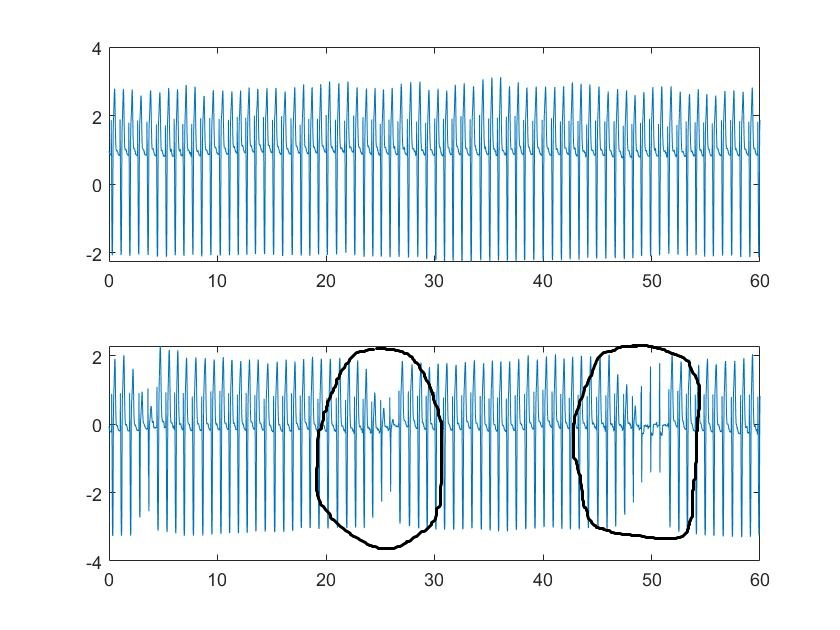
\includegraphics[width=8cm]{healthyVSunhealthy.JPG}
\caption{Healthy vs Unhealthy  ECG Signal Example}
\label{Comparison}
\end{figure}
%-------------------------------------------------------------------------
\section{Previous Works}
ECG signals have been traditionally been used to identify cardiovascular abnormalities present in the human body. However, pure ECG signals are hard to come by due to the fact that breathing pattern frequencies or electrical interferences corrupt the signal to a great extent. As a result, traditional approaches have relied on several pre-processing to actually make the signal worthy of inputting it further into data processing systems. Two types of abnormalities corrupt the ECG signals, the first one being the baseline wandering and the next one being noise. 

\begin{figure}[htbp]
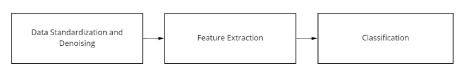
\includegraphics[width=8cm]{traditional.png}
\caption{Conventional method process}
\label{Conventional Method}
\end{figure}

Baseline wandering is an artifact present in an ECG signal and the causes for baseline wandering are the respiration of the patient and movement while recording the ECG. These make the signal hard to interpret as there might be additional frequencies other than the desired heart rate frequency alone. The traditional method of removing the baseline wandering is passing the signal into a high pass filter\cite{Alpher05}. Paper has a section that talks about many such filtering methods for removing baseline wandering.\\
\begin{figure}[htbp]
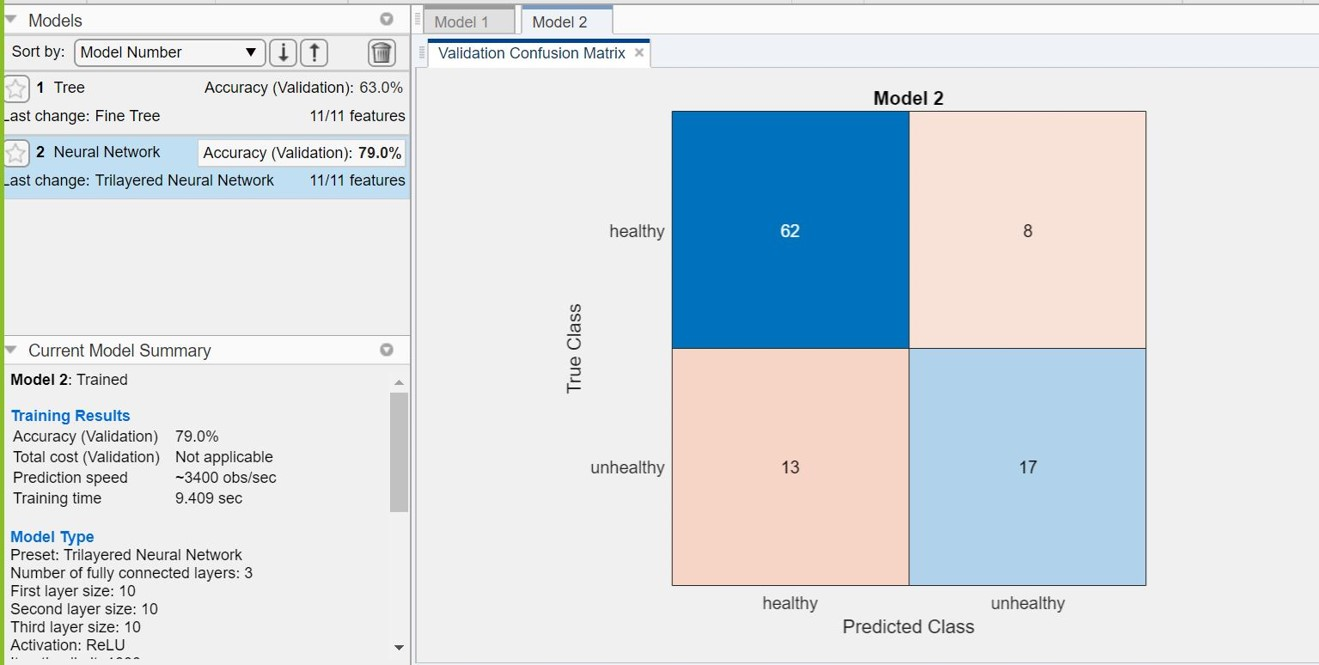
\includegraphics[width=8cm]{ConventionalResult.jpg}
\caption{Conventional method's accuracy}
\label{Classification using conventional approach}
\end{figure}
Noise in an ECG signal creeps into the ECG recording if the recording pads are not kept properly, Electromyographic noise, and power line interferences. These noises can be removed by utilizing a low pass notch filter at 50/60Hz usually.  But [Cite 1] also suggests further developments that have been used to remove the noise more efficiently.
Once the pre-processing is done, different ways are used to extract features which are then fed into the classifier. A classic feature extraction method is the Fourier transform method, peak detection( P-QRS-T wave detection). Except for the Fourier transform technique, other techniques mainly rely on time-based abnormality detections.  In the Peak detection technique, the distance between the peaks acts as the main classification basis which is computed as the distance between two R points in the P-QRS-T wave [cite 2]. A simple method of classification is the Principle component analysis of the signal itself though which the classifier will handle by itself. For frequency-based features, performing the FFT followed by the classification based on FFT coefficients is traditionally simple and gives the frequency-based feature classification.\\
We simulated the simplistic conventional model and we have presented the classifier output accuracy as shown in Figure 3.


\section{Proposed Approach}

In our proposed approach, we use DWT and WPD to perform the feature extraction step instead of using conventional feature extraction methods for ECG signals.\\
The concept of wavelet transform can be explained simply as decomposing or transforming a signal into multiple orthogonal basis functions\cite{Alpher04}. However, the difference between Fourier transform and wavelet transform or decomposition is the fact that Fourier provides resolution in frequency domain alone whereas wavelets act like a hierarchical setup of basis functions across time, where we can point out which frequency is present in what time to a considerable extent. As shown in figure 4, DWT decomposes the signal into high pass and low pass sections and as the scales go beyond 1, it takes the low pass functions alone to further look deep into its components. As seen in Figure 5, the main difference between discrete Wavelet transform and Wavelet packet decomposition stems from what these techniques decompose and look further. Wavelet packet decomposition takes both the lowpass and highpass components and decomposes them into further lowpass and highpass, thus providing a higher overall resolution of the complete signal. Thus, Wavelet packet transform results in equal-width sub-band filtering of signals as opposed to the coarser band filtering found in DWT.
\begin{figure}[htbp]
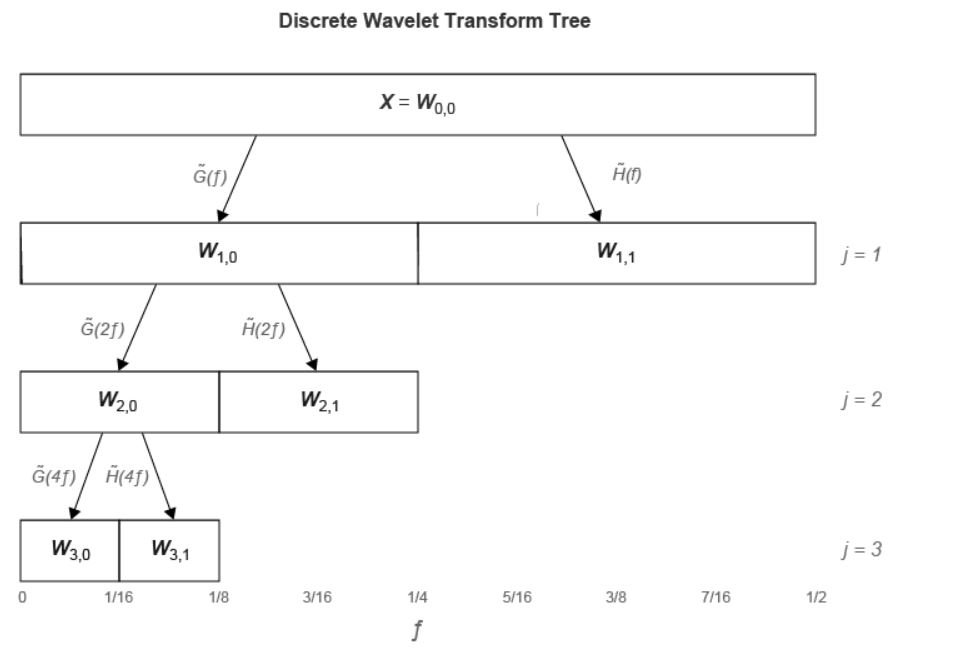
\includegraphics[width=8cm]{dwt.JPG}
\caption{frequency domain scaling representation of DWT}
\label{DWT}
\end{figure}

\begin{figure}[htbp]
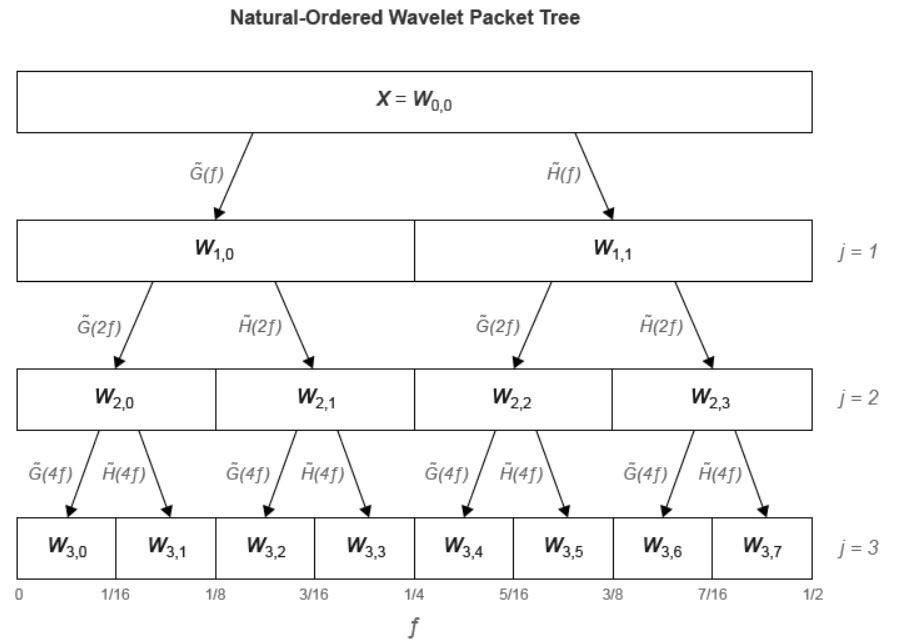
\includegraphics[width=8cm]{wpd.JPG}
\caption{frequency domain scaling representation of WPD}
\label{WPD}
\end{figure}

%\cite{Alpher01,Alpher02,Alpher03,Alpher04, Alpher05}
%Comparison experiment variables - Mother Wavelet type (Haar, DB, Symlet), Scale of DWT/WPD, Type of Decomposition (WPD or DWT).\\
By using these two approaches, we aim to optimize the accuracy of the classifier and also provide better (workable) prediction results for low-computational classifiers \cite{Alpher02}. Paper \cite{Alpher03}  takes DWT and uses a similar classification approach. Apart from the optimization that this method provides, feature extraction using this method also eliminates the need for noise removal in the data pre-processing step, thus, we can say that using this technique still keeps the classification process immune to non-linearities of the signal even after removing the noise filtering process in the data pre-processing step.
\begin{figure}[htbp]
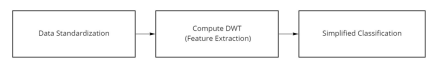
\includegraphics[width=8cm]{proposed.png}
\caption{Proposed Algorithm Flow}
\label{Proposed Algorithm}
\end{figure}

The mentioned Non-linearities of ECG signals like powerline interference will not impact the classification result while using the wavelet transform for feature extraction because when we select the features obtained from wavelet decomposition, we would ignore the data present in trivial frequency bands (containing non-essential data/ noise) and we would not feed that non-essential data to the classifier, thus denoising can be done at the feature extraction step itself.\\ 
Once we are done with the basic data pre-processing like baseline wandering removal, we need to compute the DWT/WPD coefficients for all scales. After calculating the DWT approximate and detailed coefficients, we use the selected scales of data that are best suited for our classification requirements. We take the coefficients of the selected scale and we divide the coefficients’ data into smaller chunks and calculate the energy content of each such chunk. Once we have the energy values of these chunks, we calculate the distribution of energy in these chunks and give that as an input parameter to the classifier. The classifier then takes these parameters as input from every such scale which was selected by us and runs the respective classification algorithm. We then compare the obtained results from the ones obtained from the traditional classification methods.\\
In WPD, for feature extraction purposes, \cite{Alpher01} had a good idea about using all the coefficients of the last scale of decomposition. Using this idea as the base, we checked the energy percentage distribution across coefficients and found that most of the energy was concentrated around 1-16 indexes. We have used these distribution parameters as our feature extraction pivots and have classified the healthy and unhealthy data sets.\\
We will perform a comparative study for determining which type of mother wavelet is best suited for this application and up to what scale (levels) of cascading DWT/WPD is useful for this process. furthermore, we would also check if the features extracted using wavelet packet decomposition (WPD) give better results than DWT.

\section{Simulation Results, Comparison \& Discussion}
In this section, we will discuss the experimental setup , results and discuss the observations from the classifier output.
\subsection{Simulation Environment}
The simulation environment consisted of us extracting the data from [repo link] which consist of patients with various heart arrhythmia. Each data was of length 30 mins. So in order to reduce the computationally convenient and add more data, we chose to take individual sections of the ECG that had problems as our unhealthy signal and portions of ECG signal that did not have any arrhythmia as healthy ones. Each of the unhealthy and healthy signal lengths lasted for a minute. We then used the input signal after doing pre-processing to get the features that we have mentioned above and fed it into the classifiers to see the performance.

\subsection{Simulation Results} 
We ran the simulation for 5 types of wavelets and depending on the type of method used DWT/WPD, we chose scales. Scales of 9 and 10 were used for DWT and scales of 5 and 9 were used for WPD. Table 1 and Table 2 show us the accuracy results of the classification for a particular type of classifier.

\begin{figure}[h!]
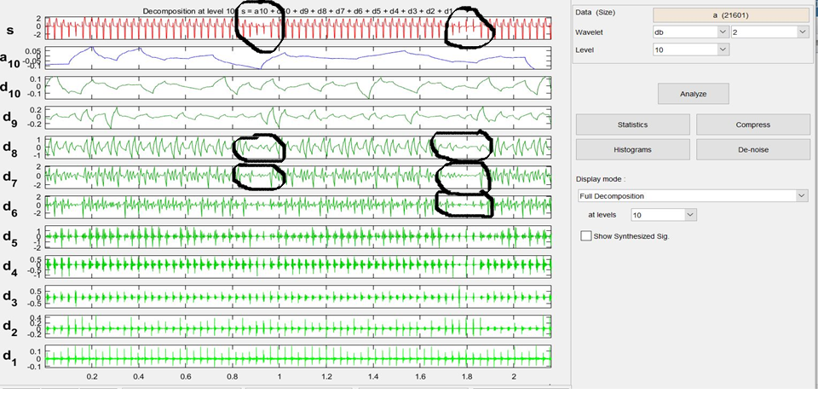
\includegraphics[width=8.5cm, height=6cm]{DWT_example.png}
\caption{Decomposition of original signal using DWT}
\label{DWT Simulation}
\end{figure}
As we can see in figure 7, the arrhythmia in the ECG signal can easily be detected using scales 6,7, and 8 of DWT decomposition, and the rest of the coefficients in other scales are not of much use to our classifier, so we would use the data only from the given scales for classification in case of DWT.\\
\begin{figure}[h!]
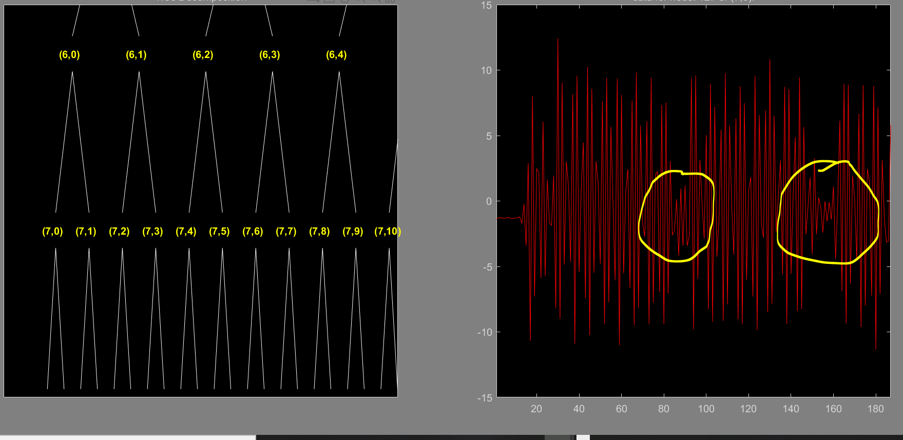
\includegraphics[width=8.5cm, height=6cm]{WPD_example.png}
\caption{Decomposition of original signal using WPD \\ node - (7,1)}
\label{WPD Simulation}
\end{figure}
Similarly in Figure 8, we visualize wavelet packet decomposition and observe that a few nodes (here - 7,1) show much more pronounced differentiation between normal and abnormal ECG signals, and similar to our method in DWT feature extraction, here we would only consider a few important nodes which are supposed to give better results.\\
\begin{figure}[h!]
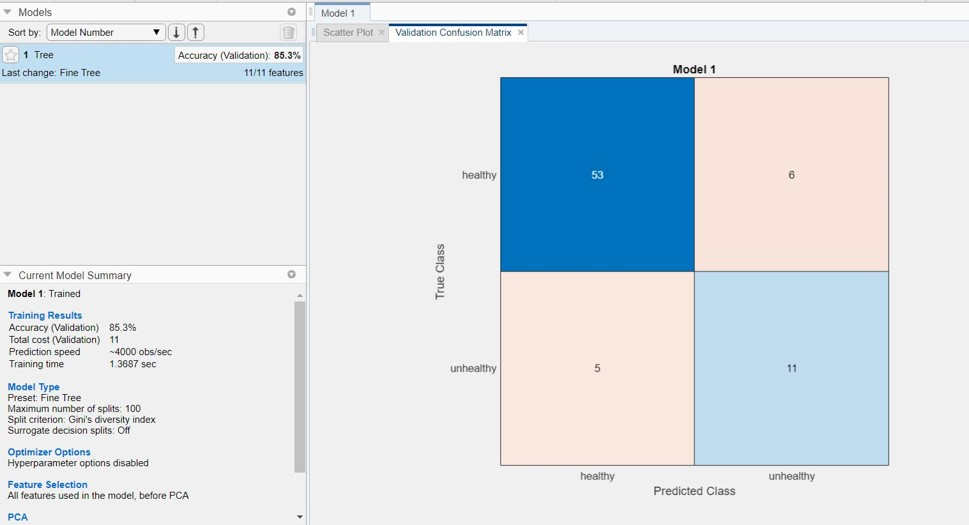
\includegraphics[width=8.5cm]{DWT_result_db2.jpg}
\caption{Classifier Output when using DWT \\ (here mother wavelet Db2) based feature extraction}
\label{DWT Simulation}
\end{figure}

\begin{figure}[htbp]
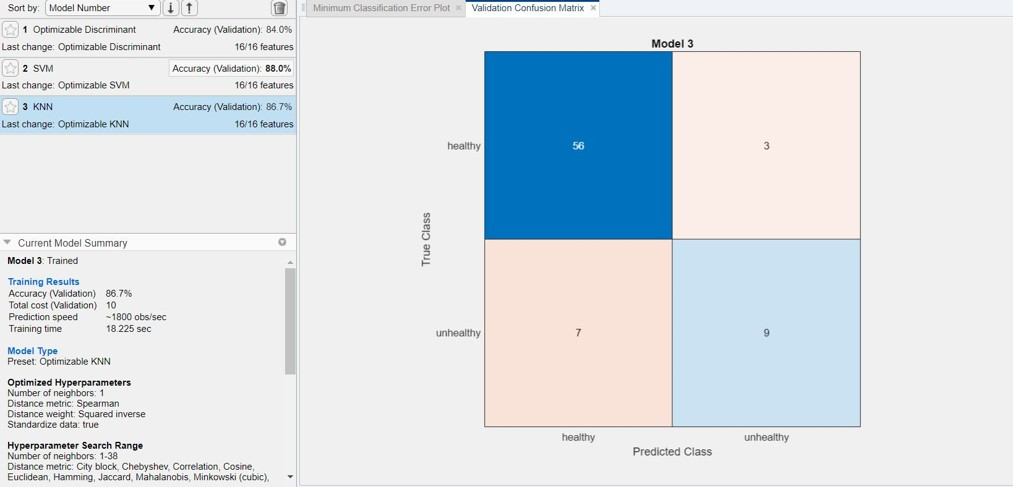
\includegraphics[width=8.5cm]{WPD_result_db6.jpg}
\caption{Classifier Output when using WPD \\ (here mother wavelet Db6) based feature extraction}
\label{WPD Simulation}
\end{figure}
Using these two techniques we give this extracted features data as an input to various classifiers which produce the confusion matrices as shown in figures 9 \& 10. From this result, we see that we get around 85\% \& 88\% classification accuracy. Similarly, we ran this simulation setup for various mother wavelets with varying scales on different classifiers and compared the results to select the best possible combination - (feature extraction type, wavelet, scale, classifier)
\subsection{Comparison \& Discussion}

As we can see from the results, in general, the classification accuracy of using WPD feature extraction is better than using DWT even at lower scales. This result was expected because of the fact that WPD will have more information when compared to the DWT of the same scale. \\
As observed in Table 1, when using DWT as a feature extraction method we have to use a scale up to 9 \& 10 for getting a reasonable classification result. When we chose mother wavelets like Haar and Symlets, we see the classification accuracy is not as good as Daubechies mother wavelets. Specifically, db2 provides the best accuracy at both scales 9 and 10, with accuracy reaching 86\% at scale 10. Now, observing the accuracy results improvement across scales, we see that there is a decent increment in the accuracy when we use higher scales like scales 8-10, but if we further increase the number of levels, the classification accuracy would start saturating due to the non-availability of meaningful samples as it is too down-sampled.
%% --------------%%
\begin{table}[htbp]
\scalebox{0.9}{
\begin{tabular}{|c|cc|cc|}
\hline
\begin{tabular}[c]{@{}c@{}}KNN \\ Classifier\end{tabular} & \multicolumn{2}{c|}{Scale : 9}                                                            & \multicolumn{2}{c|}{Scale : 10}                                                           \\ \hline
Method                                                    & \multicolumn{1}{c|}{\begin{tabular}[c]{@{}c@{}}Mother \\ Wavelet\end{tabular}} & Accuracy & \multicolumn{1}{c|}{\begin{tabular}[c]{@{}c@{}}Mother \\ Wavelet\end{tabular}} & Accuracy \\ \hline
\multirow{5}{*}{DWT}                                      & \multicolumn{1}{c|}{Db2}                                                       & 80       & \multicolumn{1}{c|}{Db2}                                                       & 86       \\ \cline{2-5} 
                                                          & \multicolumn{1}{c|}{Db4}                                                       & 72       & \multicolumn{1}{c|}{Db4}                                                       & 79       \\ \cline{2-5} 
                                                          & \multicolumn{1}{c|}{Db6}                                                       & 75       & \multicolumn{1}{c|}{Db6}                                                       & 84       \\ \cline{2-5} 
                                                          & \multicolumn{1}{c|}{Sym4}                                                      & 80       & \multicolumn{1}{c|}{Sym4}                                                      & 81       \\ \cline{2-5} 
                                                          & \multicolumn{1}{c|}{Haar}                                                      & 72       & \multicolumn{1}{c|}{Haar}                                                      & 70       \\ \hline
\end{tabular}}
\caption{Accuracy Comparison for DWT across varying \\ Mother Wavelets and Scales using KNN classifier}
\label{tab:caption}
\end{table}
In Table 2, we see classification accuracy results while using WPD as the feature extraction method. Here, for scales comparison, we are using scale 5 and scale 9 because we found that even scale 5 was able to match the classification accuracy of DWT. We tried to analyze the accuracy increment across higher scales. So we decided to compare scale 9 which was used in DWT to have a credible benchmark for our comparison. As we can interpret from this table the Haar and Symlets mother wavelets results are similar irrespective of the feature extraction method, however, we see that the performance of db6 yields the best results when using WPD and almost matches with db2's performance in DWT even when using just scale 5 in WPD.\\


%%----------------------------%%

\begin{table}[htbp]
\scalebox{0.9}{
\begin{tabular}{|c|cc|cc|}
\hline
\begin{tabular}[c]{@{}c@{}}KNN \\ Classifier\end{tabular} & \multicolumn{2}{c|}{Scale : 5}                                                            & \multicolumn{2}{c|}{Scale : 9}                                                            \\ \hline
Method                                                    & \multicolumn{1}{c|}{\begin{tabular}[c]{@{}c@{}}Mother \\ Wavelet\end{tabular}} & Accuracy & \multicolumn{1}{c|}{\begin{tabular}[c]{@{}c@{}}Mother \\ Wavelet\end{tabular}} & Accuracy \\ \hline
\multirow{5}{*}{WPD}                                      & \multicolumn{1}{c|}{Db2}                                                       & 80       & \multicolumn{1}{c|}{Db2}                                                       & 86       \\ \cline{2-5} 
                                                          & \multicolumn{1}{c|}{Db4}                                                       & 78       & \multicolumn{1}{c|}{Db4}                                                       & 84       \\ \cline{2-5} 
                                                          & \multicolumn{1}{c|}{Db6}                                                       & 84       & \multicolumn{1}{c|}{Db6}                                                       & 88       \\ \cline{2-5} 
                                                          & \multicolumn{1}{c|}{Sym4}                                                      & 80       & \multicolumn{1}{c|}{Sym4}                                                      & 82       \\ \cline{2-5} 
                                                          & \multicolumn{1}{c|}{Haar}                                                      & 78       & \multicolumn{1}{c|}{Haar}                                                      & 78       \\ \hline
\end{tabular}}
\caption{Accuracy Comparison for WPD across varying \\ Mother Wavelets and Scales using KNN classifier}
\label{tab:caption}
\end{table}
%% --------------------------%%
Overall, we can say that the db6 mother wavelet performs the best for our application closely followed by db2. Also, for our particular application, when using the DWT feature extraction method, we have to use higher scales like scales 9-10 to achieve decent accuracy. While we would only need a minimum decomposition scale of 5 to achieve the same accuracy in the WPD method. However, we can further increase the accuracy of the WPD method by increasing the decomposition levels up to 9-10.
%%----------------------------%%

\begin{table}[htbp]
\scalebox{0.7}{
\begin{tabular}{|c|c|c|cl|c|c|}
\hline
SVM Classifier                                                   & Scale 9  & Scale10  & \multicolumn{2}{c|}{}                                                                & Scale 5  & Scale9   \\ \hline
DWT                                                              & Accuracy & Accuracy & \multicolumn{2}{c|}{WPD}                                                             & Accuracy & Accuracy \\ \hline
\begin{tabular}[c]{@{}c@{}}Mother \\ Wavelet \\ Db6\end{tabular} & 81.4     & 85.3     & \multicolumn{2}{c|}{\begin{tabular}[c]{@{}c@{}}Mother \\ Wavelet\\ Db6\end{tabular}} & 83       & 87       \\ \hline
\end{tabular}}
\caption{SVM - Classification Accuracy : DWT vs WPD}
\label{tab:caption}
\end{table}

%%----------------------------%%

\begin{table}[htbp]
\scalebox{0.7}{
\begin{tabular}{|c|c|c|c|c|c|}
\hline
\begin{tabular}[c]{@{}c@{}}Decision Tree\\ Classifier\end{tabular} & Scale 9  & Scale 10 &                                                                  & Scale 5  & Scale 9  \\ \hline
DWT                                                                & Accuracy & Accuracy & WPD                                                              & Accuracy & Accuracy \\ \hline
\begin{tabular}[c]{@{}c@{}}Mother \\ Wavelet \\ Db6\end{tabular}   & 72       & 84       & \begin{tabular}[c]{@{}c@{}}Mother \\ Wavelet \\ Db6\end{tabular} & 82       & 83       \\ \hline
\end{tabular}
}
\caption{Decision Tree - Classification Accuracy :- \\ DWT vs WPD}
\label{tab:caption}
\end{table}
%%------------------------------%%
We also need to check these methods' efficacy with respect to different classifiers like a decision tree and Support Vector Machine (SVM), K- Nearest Neighbours (KNN). So we decided to take the best mother wavelet (in our case db6) and optimal decomposition scales of 5 \& 9 for WPD and 9 \& 10 for DWT respectively.
since we had already used KNN as the base classifier for table 1 \& 2, hence we decided to compare the accuracy results using SVM and Decision Tree.\\
As we can see from Tables 3 \& 4, the decision tree classifiers perform the best of for scale 10 DWT feature extraction. whereas, with regards to scale 5, the WPD's accuracy results are equivalent to DWT's best results. For SVM Classifiers, WPDs performance across scales is superior to DWT's performance.\\
As a result, we can say that when we are using KNN or SVM, WPD feature extraction is superior and is decomposition level agnostic, whereas in the decision tree's case for higher levels of decomposition one can opt for the DWT method of decomposition.\\
As we can infer from the above discussion, using wavelets can simplify our task of classification of ECG signals to a great extent. However, the method also comes with an additional cost of Wavelet Packet Transform time overhead. Also, for non-binary classification purposes, we need a purely adaptive method of scale and mother wavelet selection which is out of the scope of this project.


%-------------------------------------------------------------------------
\section{Conclusion}
In conclusion, we can deduce that the proposed method of feature extraction using DWT and DWD is much more computationally efficient ( for large scale data) than conventional methods (peak detection, QRS Detection), and by using this method we are able to reduce the number of features/dimensions of the data being fed to the classifier, thus it drastically reduces the latency of the classifier.
Using wavelet decomposition also doesn’t negatively affect the amount of useful information sent to the classifier that is used for classification.
We were also able to improve the accuracy of the classification results to a good extent. The resulting system is more time-efficient and the complexity of the overall system was hence reduced.
Further, we can say that this method can be easily applied in multi-class classification for detecting different types of abnormalities like arrhythmia, atrial flutter, fibrillation, etc to make the diagnosis more precise.


%%%%%%%%% REFERENCES
{\small
\bibliographystyle{ieee_fullname}
\bibliography{egbib}
}


\section*{Miscellaneous Links}
\begin{itemize}
    \item \href{https://physionet.org/content/mitdb/1.0.0/}{Open Source MIT-BIH Database}
    \item \href{https://github.com/abhishekkhare1998/EcgClassificationProject}{Project Repository}
    \item \href{https://github.com/abhishekkhare1998/EcgClassWaveletPaper}{Report Repository}
\end{itemize}



\end{document}
